\chapter{Entwicklung eines Prototypen des Benutzerkonzepts mit dem Angular-Framework}
\label{chap:prototyp}
Der Prototyp ist auf Basis des vorher entwickelten Benutzerkonzepts entwickelt. Für eine genaue Beschreibung des Benutzerkonzepts siehe Abschnitt~\ref{sec:bedienungskonzept}.

\section{Backend}
Das Backend ist mit Node.js und MongoDB entwickelt. 
Hierbei wird der Express-Server von Node.js und die Mongoose-Bibliothek von MongoDB verwendet, um eine effiziente und skalierbare Datenverwaltung zu gewährleisten.

Die Kernfunktionalitäten des Backends umfassen die Benutzerregistrierung und -verwaltung. 
In der Datei \texttt{server.js} werden die Endpunkte für die Registrierung und Anmeldung der Nutzer definiert. 
Die Datei \texttt{userModel.js} enthält das Schema für die Benutzer, welches die Felder Vorname, Nachname, E-Mail-Adresse und Passwort umfasst. 
Das Passwort wird in der \texttt{userModel.js}-Datei mithilfe der Bibliothek bcryptjs verschlüsselt, bevor es in der Datenbank gespeichert wird. 
Dies stellt sicher, dass Passwörter nicht im Klartext in der Datenbank gespeichert werden. 
 Datei \texttt{server.js} ist ebenfalls für die Überprüfung zuständig, ob ein Nutzer existiert und ob seine Anmeldedaten korrekt sind. 
 Dies ermöglicht eine sichere Authentifizierung der Nutzer.

Die Registrierung eines neuen Nutzers erfolgt über die Methode \texttt{app.post('/api/register', async (req, res) => \{ ... \})}. 
Der Nutzer gibt seine Daten ein, und bei korrekter Eingabe wird ein neues Benutzerobjekt basierend auf diesen Eingaben erstellt. 
Über die Methode \texttt{app.post('/api/login', async (req, res) => \{ ... \})} wird beim Anmeldeversuch eines Nutzer abgeglichen, ob die eingegebenen E-Mail-Adresse und das Passwort mit den in der Datenbank gespeicherten Daten übereinstimmen. 
Zunächst wird überprüft, ob ein Nutzer mit der angegebenen E-Mail-Adresse existiert. 
Falls nicht, wird eine Fehlermeldung „Benutzer nicht gefunden“ zurückgegeben. 
Anschließend wird das eingegebene Passwort mit dem in der Datenbank gehashten Passwort verglichen. 
Ist das Passwort falsch, erhält der Nutzer die Fehlermeldung „Falsches Passwort“. 
Bei korrekter Eingabe der Anmeldedaten wird die Nachricht „Login erfolgreich“ zurückgegeben.

\section{Frontend}
Das Frontend der Anwendung ist mit dem Angular Framework entwickelt. 
Alle Seiten der Anwendung sind responsiv gestaltet, sodass die Nutzer die Anwendung sowohl auf dem Handy als auch auf dem Laptop angenehm nutzen können. 
Für den Dark Mode werden derzeit die Systemeinstellungen des Geräts verwendet.

\begin{figure}[h]
    \centering
    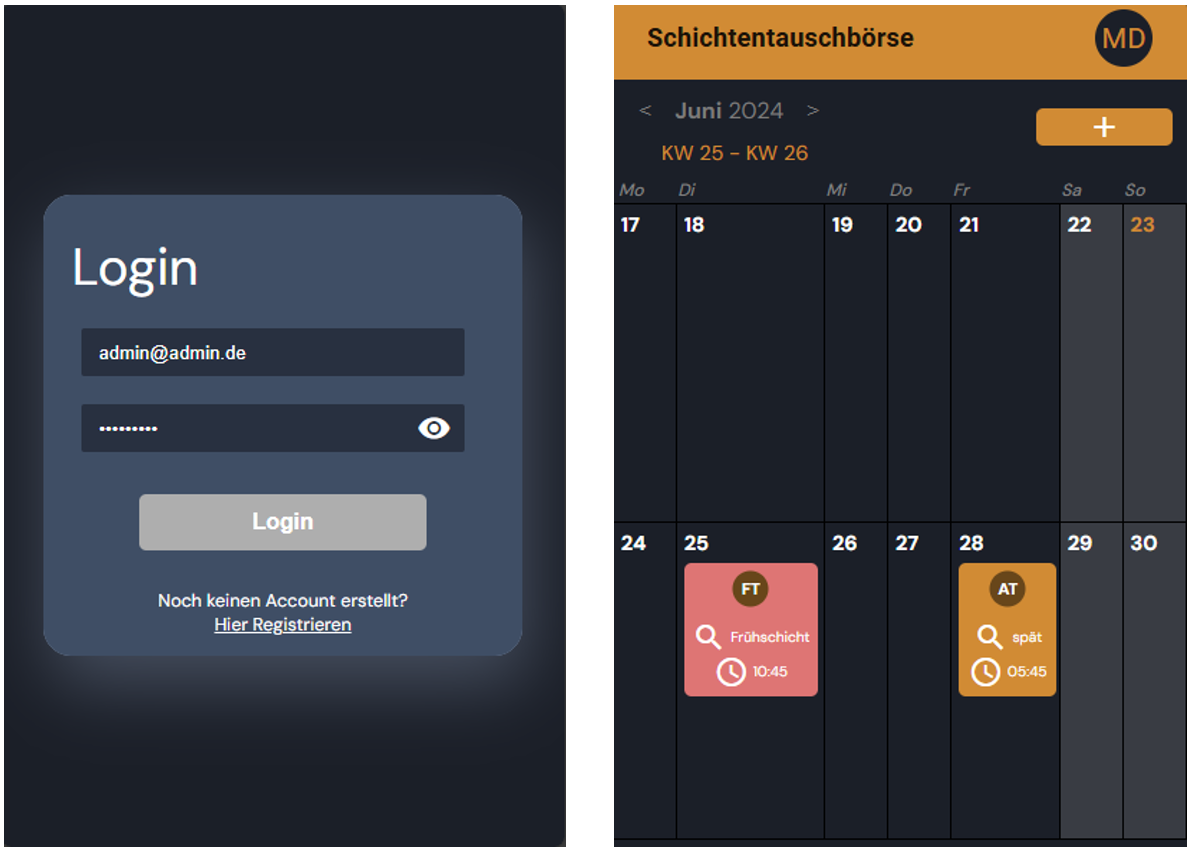
\includegraphics[clip,width=0.8\linewidth]{images/Login_Home_dark.png}
    \caption[Login- und Übersichtsseite im Dark Mode auf einem 400x600px großen Bildschirm]{Login- und Übersichtsseite im Dark Mode auf einem 400x600px großen Bildschirm}
    \label{Login_Home_dark}
\end{figure}

Wenn ein Nutzer die Anwendung zum ersten Mal benutzt, muss er sich zunächst registrieren. 
Die Eingabefelder für die Registrierung werden validiert, um sicherzustellen, dass beispielsweise die E-Mail-Adresse im richtigen Format eingegeben wird. 
Mit der \texttt{PasswordStrengthValidator()} Funktion wird überprüft, ob das Passwort sicher genug ist. 
Da der Nutzer das Passwort zur Überprüfung zweimal eingeben muss, wird mithilfe der \texttt{passwordMatchValidator()} Funktion sichergestellt, dass beide Passwörter übereinstimmen. 
Falls dies nicht der Fall ist, wird eine Fehlermeldung angezeigt. 
Über das Augensymbol im Eingabefeld kann der Nutzer sich jedoch seine Passwörter anzeigen lassen (siehe Login-Seite in Abbildung \ref{Login_Home_dark}).

Der Service \texttt{user.service.ts} kommuniziert für Login und Registrierung über HTTP-Anfragen mit dem Express-Server im Backend. 
Nach erfolgreicher Registrierung wird der Nutzer zum Login-Formular weitergeleitet, wo er sich mit seinem erstellten Account anmelden kann. 
Wenn die Anmeldedaten korrekt sind, wird der Nutzer zur Übersichtsseite weitergeleitet, von der aus alle anderen Seiten erreichbar sind.

Die Felder, in denen ein Tauschangebot eingetragen ist, sind etwas breiter, damit die Informationen besser zu erkennen sind. 
Der heutige Tag ist farbig hervorgehoben, wie in Abbildung \ref{Login_Home_dark} zu sehen ist.

Zusätzlich kann sich der Nutzer in den Einstellungen auch wieder ausloggen. Hierfür wird die Funktion \texttt{logout()} aus der \texttt{auth.service.ts}-Datei verwendet. 
Eine Funktion zum Exportieren der Tauschangebote in den Kalender wird im Frontend bereits angezeigt, ist jedoch im Backend noch nicht implementiert.

Wenn der Nutzer auf der Übersichtsseite auf den Button mit dem Plus klickt, kann er eine neue Tauschanfrage erstellen, die Eingabefelder dafür verwenden Angular Material. 
Der Nutzer kann das Datum aus einem Kalender auswählen oder selbst eingeben. Die angebotene und gesuchte Schicht kann aus einem Dropdown-Menü ausgewählt werden. 
Wenn der Nutzer eine benutzerdefinierte Uhrzeit eingeben möchte, kann er "Benutzerdefinierte Uhrzeit" auswählen. 
Dann erscheint ein neues Eingabefeld, in dem er diese Uhrzeit eintragen kann. Durch Angular Material wird sichergestellt, dass die Uhrzeit im richtigen Format eingegeben wird. 
Eine Anfrage kann nur abgeschickt werden, wenn mindestens das Datum sowie die angebotene und gesuchte Schicht eingetragen sind.

Durch Klicken auf ein Tauschangebot im Kalender (siehe Abbildung \ref{Login_Home_dark}) öffnet sich eine Seite mit detaillierteren Informationen, je nachdem, welche Informationen für die Schicht relevant sind und vom Nutzer eingetragen wurden.